\chapter{Gestione delle risorse e design}\label{ch:gestionerisorse}

Riuscire ad ottimizzare il caricamento delle risorse, come fogli di stile CSS, 
e mantenere un design coerente in tutti i sottoprogetti sono due
 grandi sfide della programmazione microfrontend, ne vediamo quindi delle strategie.


\section{Caricamento delle risorse}
Possono essere presenti nei progetti dei fragments dei file CSS e javascript, necessari
al giusto design e funzionamento logico del componente. Esistono diverse politiche 
atte a caricare le risorse necessarie a tutti i microfronend:

\subsection{Referencing con soluzioni client-rendered}
Il modo più semplice consiste nel caricare le risorse necessarie direttamente nell'HTML della pagina ospitante.
I team quindi dovranno fornire gli indirizzi dei file richiesti.
Per far risparmiare traffico agli utenti, di solito viene impostata una regola che fa mantenere ai client
le risorse in cache per un anno, in questo modo non devono essere scaricate tutte le volte.

Ma quando viene distribuito un aggiornamento di un file, i client hanno in cache delle versioni obsolete, e devono riscaricarle.
Per far si che avvenga, si appone al nome dei file il \textbf{fingerprint}, un codice alfanumerico che deriva dal checksum del file.
Questa tecnica, chiamata \textbf{cache busting}, forza il browser dell'utente a riscaricare i file quando questi vengono modificati,
ovvero quando il loro fingerprint cambia.
\\\\
Per far si che i team possano distribuire autonomamente i file, senza comunicare ogni volta il nuovo nome del
fingerprint alla pagina ospitante, si include in questa dei nomi generici, che verranno poi reindirizzati dal webserver all'ultimo file aggiornato.



\subsection{Referencing con soluzioni server-rendered}
Se il progetto utilizza già il rendering server-side, è possibile includere le risorse nel codice
del fragment, in modo che quando questo viene sostituito con un comando SSI dal webserver, vada ad includere
nella pagina HTML anche i file necessari. Se però il fragment viene incluso nella pagina più volte, anche le risorse vengono 
scaricate ripetutamente. Inoltre i file javascript vengono eseguiti tante volte quanto vengono inclusi nella pagina,
il che va ad aumentare il carico sulla CPU del client e il crearsi di errori di esecuzione.


\subsection{I vantaggi di HTTP/2}
Il nuovo protocollo HTTP/2, basato sul progetto SPDY sviluppato da Google nel 2009, estende il precedente HTTP/1
aumentando la velocità di caricamento delle pagine, grazie alla riduzione dell' header HTTP.
\\\\\\
Il raggruppamento di più risorse in un'unica risposta dal server è stata un'ottimizzazione fondamentale per HTTP/1.x, in cui 
il parallelismo limitato e l'overhead elevato del protocollo in genere superavano tutte le altre preoccupazioni.
Tuttavia, con HTTP/2, il multiplexing non è più un problema e la compressione dell'intestazione 
riduce drasticamente il sovraccarico dei metadati di ogni richiesta HTTP.\cite{http2}
\\\\
Di conseguenza con l'avvento di HTTP/2, il concatenamento di richieste e la divisione delle risorse è un aspetto che non 
 va più a invalidare le prestazioni, il che significa che ora possiamo ottimizzare le nostre applicazioni fornendo risorse 
 più granulari.
 \\
 Ecco alcuni vantaggi pratici derivanti dalla più alta granuralità delle risorse con HTTP/2:

 \begin{itemize}
     \item I browser andranno a scaricare \textbf{parti di codice più piccole}, evitando di farlo per 
     quelle che non sono state modificate e che risiedono in cache. 
     Grazie a questo i team possono operare con una distribuzione continua, anche più volte al giorno.
     \item Si avranno \textbf{task di codice javascript più brevi}, che favoriranno la reattività all'input dell'utente.
     \item Si potrà facilmente far caricare all'utente le risorse necessarie esclusivamente
      a visualizzare la pagina corrente
 \end{itemize}

\pagebreak


 \section{Design system}

 Un progetto composto da microfrontend ha come priorità l’autonomia, ma tutti i pezzi del progetto devono apparire 
 all’utente come parte di una cosa sola, e devono avere delle caratteristiche visive in comune. Insomma, i team hanno 
 bisogno di un modo per condividere uno schema di design e stilizzazione.

Un design system contiene parti di design, come font, colori, icone, componenti di interfaccia riusabili, come bottoni 
e form, e anche un ben definito insieme di regole.
\\\\
Un design system ben fatto porta ai seguenti benefici:
\begin{itemize}
    \item \textbf{Consistenza:} i microfrontend appaiono familiari tra di loro agli occhi dell’utente
    \item \textbf{Linguaggio condiviso:} i team devono parlare la stessa lingua, questo porta a limitare equivoci.
    \item \textbf{Velocità di sviluppo:} avere componenti di design già pronti velocizza molto lo sviluppo di nuove features
    \item \textbf{Scalabilità}: avendo un buon design system condiviso, un nuovo team può subito adottarlo, e velocizzare lo sviluppo, niente è ridondante.
\end{itemize}
Ovviamente creare un design system porta ad un impiego importante di risorse, ma va visto come un investimento a medio-lungo termine.
\\\\
Non obbligatoriamente per un nuovo progetto si deve creare un design system proprietario.
Se il prodotto che stiamo costruendo è per uso interno di un’azienda, o non vogliamo investire troppo su una personalizzazione del design è molto meglio adottare progetti
 già realizzati, come Bootstrap o Material UI.

\subsection{sviluppo di un design system}
Ci sono due modi per sviluppare un design system, il modello centrale e quello federated:

Nel modello \textbf{centrale} un team di design, composto da UX designer, è impiegato esclusivamente per il design system. Gli altri team sono degli utilizzatori, che adottano i
 prodotti di quest'ultimo.
\\\\
I team di produzione richiedono nuovi componenti grafici e il team di design li crea. 
Possono crearsi dei rallentamenti, perche un unico team di design dovrà servire diversi team di produzione.
\\\\
Nel modello \textbf{federated} invece gli UX designer vengono inseriti nei vari team di produzione, e realizzeranno le componenti grafiche richieste dai loro colleghi. 
Ovviamente tutti i nuovi elementi creati verranno messi a disposizione anche agli altri team.
\begin{figure}[H]
    \centering
    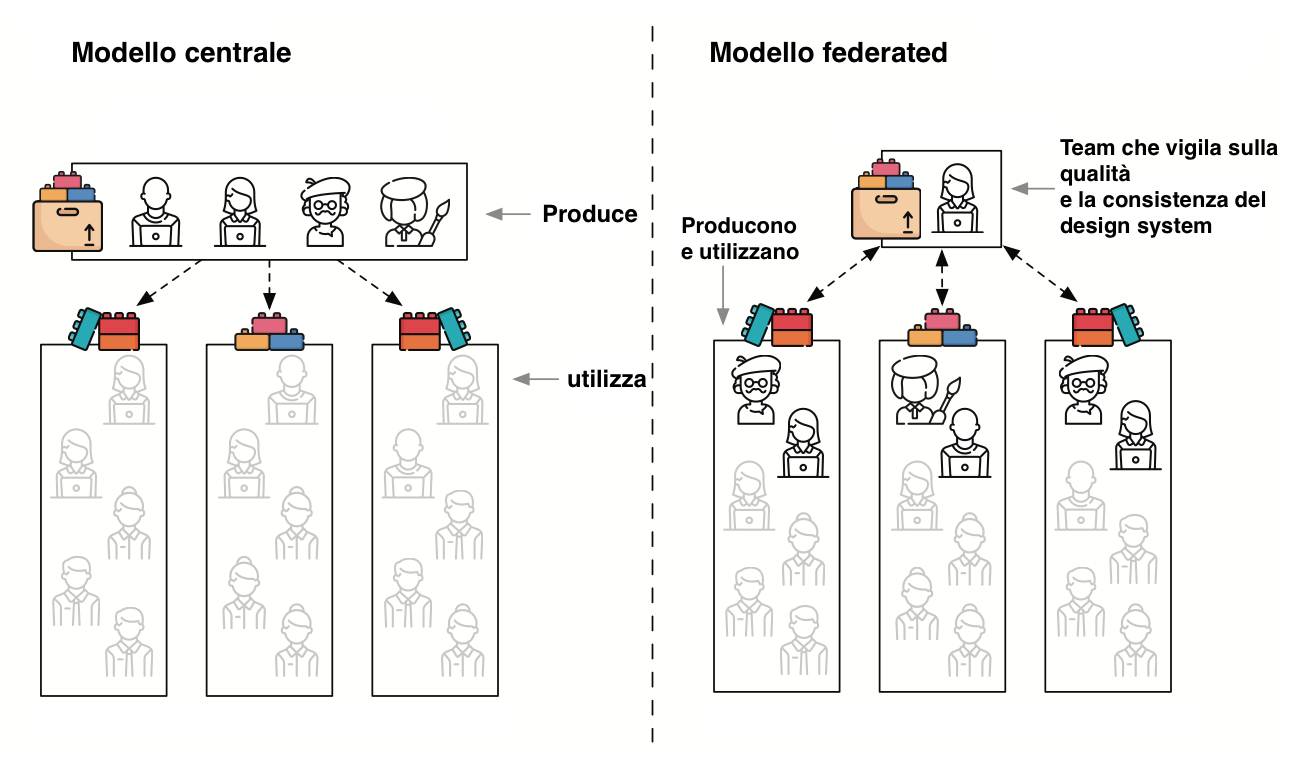
\includegraphics[width=148mm]{img/design system}
    \caption{Le principali differenze tra il modello centrale, dove un team si occupa esclusivamente del design, e
    quello federated, dove tutti concorrono alla realizzazione di questo. Il modello federated ha anche un team che si occupa di controllare la \textbf{qualità} e la 
    \textbf{consistenza} dei componenti creati.}
  \end{figure}

Spesso questi due modi di sviluppare il design system vengono usati insieme quando si inizia un nuovo progetto dove 
all'interno si crea un apposito design system: all’inizio il lavoro da fare
 è tanto, e quindi si parte con l’approccio centrale, per poi via via migrare a quello federated.